\section{Our Triplet Loss Model}
\addcontentsline{toc}{section}{Our Triplet Loss Model}
\label{sec:triplet_loss_model}

\subsection{Specific Dataset}
Since the \hyperref[sec:kagglechallenge]{Kaggle Challenge} already provides a testing mechanism, we only had to choose a validation dataset. We already disregarded more then half of individuals by now so we do not want to throw away more data. Hence, we decided to only consider individuals with $>3$ images. We then used a method very similar to the smart \hyperref[subsubsec:smart-batches]{Smart Batches Algorithm}:

\begin{enumerate}
    \item Iterate over all the individuals with $>3$ images.
    \item Take the first two images and put them to the side to make sure we don't disregard individuals.
    \item Shuffle the remaining images (with a seed).
    \item According to the split ratio $S$ (we choose $0.1$), take the first $\lceil S * len(remaining\  images) \rceil$ individuals as your validation dataset.
    \item Use all the other images as the train dataset.
\end{enumerate}

\noindent Then we called the \hyperref[subsubsec:smart-batches]{Smart Batches Algorithm} and do the remaining standard preprocessing steps. We used the seed $0$.

\subsection{Configurations and Hyperparameters}
To test our hypotheses we  will train these models:
\begin{enumerate}
    \item InceptionV3 Model with the weights pretrained on the Softmax species.
    \item InceptionV3 with imagenet weights.
    \item Resnet50V2 with imagenet weights.
\end{enumerate}

\noindent For simplicity, we will refer to the models from now on as "Species-Weights", "ImageNet-Weights" and "Control-Model". \\
As for the embedding block, which we put on top of the CNN, we choose this architecture: 3 Dense-Layers with $512$, $256$ and $256$ output neurons respectively and $ReLu$ - activation functions. We then choose to use a l2-normalizing layer as our final output layer to enforce more evenly distributed distances to then later be able to better identify new individuals. \\
We do automated online semi hard triplet mining with a default margin of $1$.

\noindent Since the the \hyperref[sec:kagglechallenge]{Kaggle Challenge} offers a nice automatic way of testing models, we had to only come up with a validation procedure for our inter-model comparison. We decided for this 2 stage validation procedure:


Since our model should learn to 1. recognize  and 2. also recognize  when it has not seen an individual before we come up with this 2 stage validation procedure:


Firstly since our model should learn to recognize individuals it has seen before, we decided to measure the accuracy of recognizing the a known individual, the k5-individual accuracy and the accuracy of classifying the right species. To achieve this we firstly we calculated the embeddings of our train and validation datasets. Then we computed the pairwise distance matrix with an euclidean metric of the two embeddings and sort out the labels with the 5 closest values. With these labels we now could calculate the beforehand mentioned accuracies. In addition we used \href{https://umap-learn.readthedocs.io/en/latest/basic_usage.html}{UMAP} to visualize a dimensional representation of our embeddings. 
Secondly our model should also recognize when it has not seen an individual before. For that we used the individuals with only one picture and calculated there embeddings. We then calculate the pairwise distance matrix of those embeddings with the train embeddings and sorted out the distance to the nearest neighbor. We then compared this distance to with the average distance of individuals which our model is already familiar with. For that we created density plots of the distributions.

\subsection{Evaluation}

\subsubsection{General Training Behaviour}

\begin{figure}[ht] 
        \centering 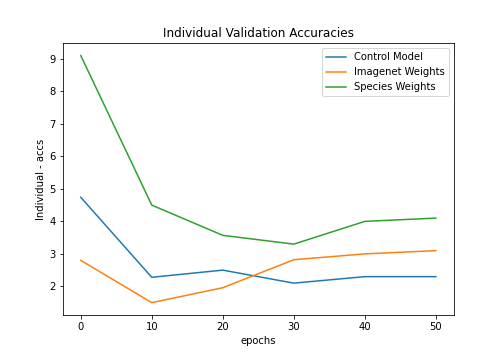
\includegraphics[width=1\columnwidth]{figures/sieamesevalacc.png}
        \caption{\label{fig:sialoss} Individual Validation Accuracies}
\end{figure}When looking at these results in Figure 7 we were really confused at first. Why does every Model has it's best performance before training? After doing some did some data-analysis we had this idea: Before training all the weights of our embedding block are randomly initiated. Thus a high Validation Acuraccies arises probably from the very uneven distribution of individual counts. First we have to look at the dataset which we use for our siamese model training and validation, the dataset containing all the individuals with at least 2 images. The top 300 individual of this data, make out 5\% of all individuals and 40\% of all images. So if we know choose to random images from the data the chances of getting the same individual are quite high.
Interesting is now the composition to which species these individuals belong:
\begin{figure}[ht] 
        \centering 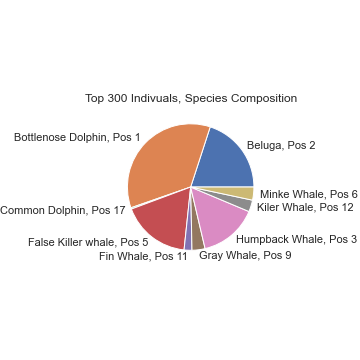
\includegraphics[width=1\columnwidth]{figures/compo.png}
        \caption{\label{fig:compo} Species Composition of top 300 Indivuals. \textit{Pos} refers to the degree of frequency}
\end{figure}\\
In addition what is very interesting is that the species accuracy, the likehood of the next neighbor in the embedding space, is for all models around around 80\% after epoch 30. If we combine this with the fact that the top 300 individuals belong mainly the most frequent species, we can refer that the most frequent classes are quite densely packed together in the embedding space. This would mean that most images are in densely packed spheres. We assume that therefore we have a lot "Hard-Triplet-Pairs" in within these spheres of the most frequent species. In addition the 2d UMAP-plots of our embeddings support these hypothesis.

\subsubsection{Species Weights vs Imagenet Weights}
All the 3 validation accuracies (Individual, k5-Individual, Species) and also the 2d-UMAP-plots before and while training show that the Species Weights Model performs significantly compared to the Imagenet-Model.


\subsubsection{Species Weights vs Imagenet Weights}
All the 3 validation accuracies (Individual, k5-Individual, Species) and also the 2d-UMAP-plots before and while training show that the Species Weights Model performs significantly compared to the Imagenet-Model.

\subsubsection{Imagenet Weights vs Control Model}
Although the InceptionV3 Model outperforms the Resnet50V2 model in terms Individual and k5 accuracy the effect is by far not as strong in the Softmax case. Especially if we into account that it took the InceptionV3 model almost double as long as the Control Model to have a convergent training loss. 

\subsection{Kaggle Test Dataset Evaluation}
Since our best performing model is quite ironically the Species-Model before training even one epoch with the triplet loss, we choose it for the test evaluation. 
To now test our model we had to create a submission.csv according to \href{https://www.kaggle.com/competitions/happy-whale-and-dolphin/overview/evaluation}{this guidelines}.
Most importantly is that we not only have to identify individuals which we have seen before, but also new individuals. 
For that we used the \href{https://drive.google.com/uc?id=1syxxE7cTRHr7iRN7vo19Wp3ewCINJxEg}{density plot} of the average distance of new individuals to the their next neighbors compared to known individuals. Looking at the distributions we decided to expect there to be a new individual at a distance of $0.35$. 
To generate the submission.csv we now first had to compute the embeddings of all our data (the Kaggle training data) and the embeddings of the Kaggle test data. Then we computed the pairwise distance matrix and sorted out the 5 closest neighbors and their corresponding labels. For every test image we know iterated through the list of the 5 closest neighbors. If the distance to the neighbor was bigger then $0.35$ we inserted "new\_individual" into the list at that position. Like this we achieved a score of $0.077$.
